% =====================================================================
%  CISC-8 Processor -- Requirements Specification
%  Build:  pdflatex main.tex  (run twice for TOC and references)
%     or:  latexmk -pdf main.tex
% =====================================================================
\documentclass[11pt,a4paper]{article}
\providecommand\SuspendTagging[1]{}
\providecommand\ResumeTagging[1]{}

% ---------------------------------------------------------------------
%  Packages
% ---------------------------------------------------------------------
\usepackage[T1]{fontenc}
\usepackage[utf8]{inputenc}
\usepackage{lmodern}
\usepackage{microtype}
\usepackage[a4paper,margin=2.3cm,headheight=14pt]{geometry}
\usepackage{amsmath}
\usepackage{array}
\usepackage{booktabs}
\usepackage{tabularx}
\usepackage{xltabular}
\usepackage{enumitem}
\usepackage{xcolor}
\usepackage{listings}
\usepackage{fancyhdr}
\usepackage{lastpage}
\usepackage{caption}
\usepackage{needspace}
\usepackage{tikz}
\usetikzlibrary{arrows.meta,calc,positioning,decorations.pathreplacing}
\usepackage[hidelinks]{hyperref}

% ---------------------------------------------------------------------
%  Document metadata -- edit here
% ---------------------------------------------------------------------
\newcommand{\DocTitle}{CISC-8 Processor}
\newcommand{\DocSubtitle}{Requirements Specification}

\newcommand{\DocVersion}{0.1 (draft)}
\newcommand{\DocDate}{8 November 2026}
\newcommand{\DocAuthor}{Michal Lagosz}

% ---------------------------------------------------------------------
%  Colours and styles
% ---------------------------------------------------------------------
\definecolor{accent}{HTML}{2F6FDB}
\definecolor{lineclr}{HTML}{8C8C80}
\definecolor{tint}{HTML}{F1F1EC}

\lstset{
  basicstyle=\ttfamily\small,
  columns=fullflexible,
  keepspaces=true,
  frame=single,
  rulecolor=\color{lineclr},
  xleftmargin=1em,
  framexleftmargin=0.5em,
  commentstyle=\color{black!55},
  morecomment=[l]{;},
}

\setlist{itemsep=2pt,topsep=4pt}
\captionsetup{font=small,labelfont=bf}
\setlength{\parindent}{0pt}
\setlength{\parskip}{6pt}
\renewcommand{\arraystretch}{1.25}

% ---------------------------------------------------------------------
%  Requirement macros
% ---------------------------------------------------------------------
% Requirement keywords (RFC 2119 style)
\newcommand{\MUST}{\textbf{MUST}}
\newcommand{\MUSTNOT}{\textbf{MUST NOT}}
\newcommand{\SHOULD}{\textbf{SHOULD}}
\newcommand{\MAY}{\textbf{MAY}}

% Requirements table:
%   \begin{reqtable}
%     \req{ARCH-001}{The processor \MUST ...}
%   \end{reqtable}
\newenvironment{reqtable}{%
  \par\small
  \xltabular{\linewidth}{@{}>{\ttfamily}p{2.1cm}X@{}}
  \toprule
  \normalfont\bfseries ID & \bfseries Requirement \\
  \midrule
  \endfirsthead
  \toprule
  \normalfont\bfseries ID & \bfseries Requirement (cont.) \\
  \midrule
  \endhead
  \bottomrule
  \endfoot
}{%
  \endxltabular
}
\newcommand{\req}[2]{\leavevmode\phantomsection\label{req:#1}#1 & #2 \\}
% Cross-reference to a requirement by its ID (clickable): \reqref{ISA-040}
\newcommand{\reqref}[1]{\hyperref[req:#1]{\texttt{#1}}}

% Shorthand
\newcommand{\IIC}{I\textsuperscript{2}C}
\newcommand{\reg}[1]{\texttt{#1}}
\newcommand{\hex}[1]{\texttt{0x#1}}

% ---------------------------------------------------------------------
%  Header / footer
% ---------------------------------------------------------------------
\pagestyle{fancy}
\fancyhf{}
\fancyhead[L]{\small\DocTitle{} -- \DocSubtitle}
\fancyfoot[C]{\small Page \thepage{} of \pageref{LastPage}}
\renewcommand{\headrulewidth}{0.4pt}

% =====================================================================
\begin{document}

% ---------------------------------------------------------------------
%  Title page
% ---------------------------------------------------------------------
\begin{titlepage}
  \centering
  \vspace*{3cm}
  {\Huge\bfseries \DocTitle\par}
  \vspace{0.6cm}
  {\LARGE \DocSubtitle\par}
  \vspace{0.4cm}
  {\large 8-bit CISC processor with Harvard architecture,\\
   windowed register file and native \IIC{} controller\par}
  \vspace{2.5cm}
  \begin{tabular}{@{}ll@{}}
    \toprule
    Date            & \DocDate \\
    Author          & \DocAuthor \\
    \bottomrule
  \end{tabular}
\end{titlepage}

\tableofcontents
\listoffigures
\newpage

% ---------------------------------------------------------------------
%  Body
% ---------------------------------------------------------------------
% =====================================================================
\section{Introduction}
\label{sec:intro}
% =====================================================================

This document specifies the requirements for CISC-8: an 8-bit CISC processor
with a Harvard architecture, 64 general-purpose registers accessed through a
sliding window of 8 registers, and a hardware \IIC{} controller. It is the
baseline for the RTL design.

\subsection{Conventions}

Every requirement has a unique identifier of the form \texttt{PREFIX-NNN} and
is verifiable. The following keywords define the weight of a requirement:

\begin{center}
\small
\begin{tabularx}{\linewidth}{@{}lX@{}}
  \toprule
  \textbf{Keyword} & \textbf{Meaning} \\
  \midrule
  \MUST{} / \MUSTNOT & Mandatory; failure to comply is a non-conformance. \\
  \SHOULD & Recommended; any deviation must be justified in the design documentation. \\
  \MAY & Optional; left to the implementer. \\
  \bottomrule
\end{tabularx}
\end{center}

Prefixes: \texttt{ARCH} (general architecture), \texttt{MEM} (memory),
\texttt{REG} (registers), \texttt{SFR} (special function registers),
\texttt{ISA} (instructions), \texttt{I2C} (\IIC{} controller),
\texttt{INT} (interrupts and reset), \texttt{IO} (interfaces),
\texttt{NF} (non-functional).

Hexadecimal numbers are written with the prefix \texttt{0x}, binary numbers
with \texttt{0b}. Bit 0 is the least significant bit (LSB).


% =====================================================================
\section{Architecture overview}
\label{sec:overview}
% =====================================================================

CISC-8 is a core with two independent memory buses (Harvard), a 64-register
file visible through the window R0--R7, and peripherals (\IIC, interrupts)
accessed through the SFR address space (Figure~\ref{fig:block}).

\begin{figure}[htbp]
  \centering
  % ---------------------------------------------------------------------
%  CISC-8 block diagram
%  Coordinates are in "units" (1 unit = 0.19 mm), y grows downwards.
%  \cpublk{style}{x}{y}{w}{h}{name}{line 1}{line 2}
% ---------------------------------------------------------------------
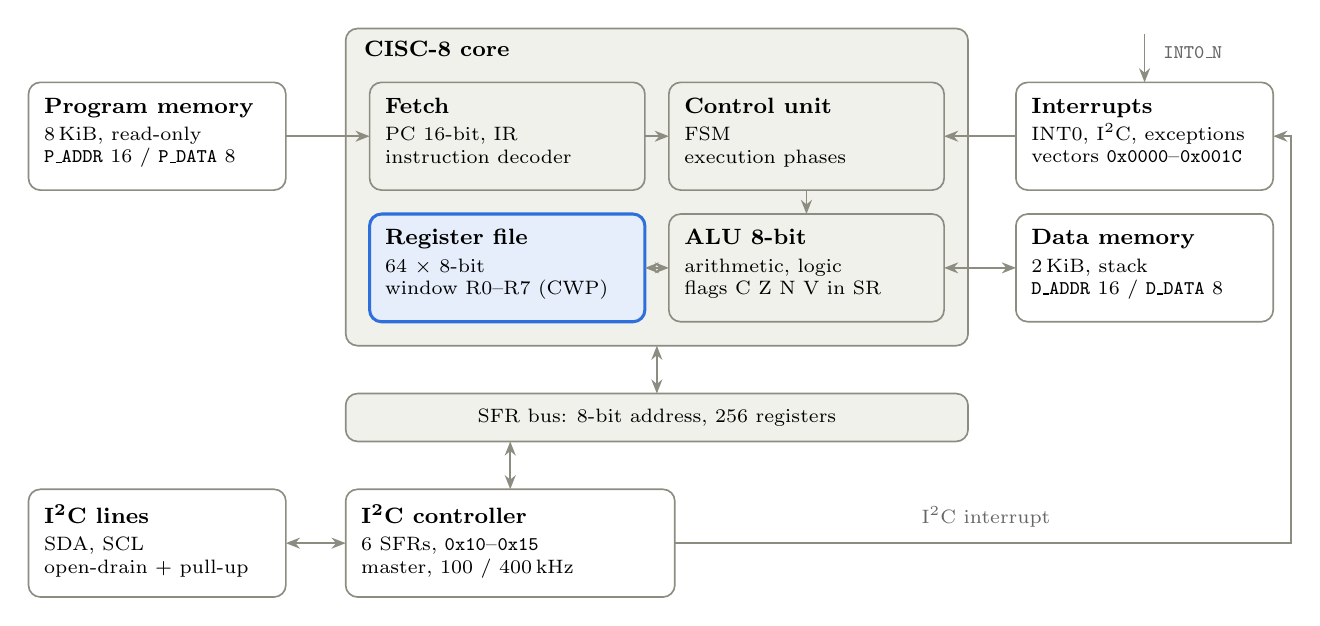
\begin{tikzpicture}[
    x=0.19mm, y=-0.19mm,
    >={Stealth[length=1.8mm,width=1.4mm]},
    blk/.style={draw=lineclr, rounded corners=1.5mm, line width=0.6pt},
    hl/.style={draw=accent, fill=accent!12, rounded corners=1.5mm, line width=1.1pt},
    grp/.style={draw=lineclr, fill=tint, rounded corners=1.5mm, line width=0.6pt},
    conn/.style={draw=lineclr, line width=0.6pt},
    lbl/.style={font=\scriptsize, text=black!60},
  ]
  \newcommand{\cpublk}[8]{%
    \draw[#1] (#2,#3) rectangle ++(#4,#5);
    \node[anchor=north west, align=left, inner sep=0pt, font=\scriptsize]
      at (#2+10,#3+10) {\textbf{\footnotesize #6}\\[2pt]#7\\#8};
  }

  % --- core container -------------------------------------------------
  \draw[grp] (212,52) rectangle ++(416,212);
  \node[anchor=north west, inner sep=0pt, font=\footnotesize\bfseries]
    at (224,60) {CISC-8 core};

  % --- blocks ---------------------------------------------------------
  \cpublk{blk}{0}{88}{172}{72}{Program memory}{8\,KiB, read-only}{\texttt{P\_ADDR} 16 / \texttt{P\_DATA} 8}
  \cpublk{blk}{228}{88}{184}{72}{Fetch}{PC 16-bit, IR}{instruction decoder}
  \cpublk{blk}{428}{88}{184}{72}{Control unit}{FSM}{execution phases}
  \cpublk{blk}{660}{88}{172}{72}{Interrupts}{INT0, \IIC, exceptions}{vectors \hex{0000}--\hex{001C}}
  \cpublk{hl}{228}{176}{184}{72}{Register file}{64 $\times$ 8-bit}{window R0--R7 (CWP)}
  \cpublk{blk}{428}{176}{184}{72}{ALU 8-bit}{arithmetic, logic}{flags C Z N V in SR}
  \cpublk{blk}{660}{176}{172}{72}{Data memory}{2\,KiB, stack}{\texttt{D\_ADDR} 16 / \texttt{D\_DATA} 8}
  \cpublk{blk}{212}{360}{220}{72}{\IIC{} controller}{6 SFRs, \hex{10}--\hex{15}}{master, 100 / 400\,kHz}
  \cpublk{blk}{0}{360}{172}{72}{\IIC{} lines}{SDA, SCL}{open-drain + pull-up}

  % --- SFR bus --------------------------------------------------------
  \draw[grp] (212,296) rectangle ++(416,32);
  \node[font=\scriptsize] at (420,312) {SFR bus: 8-bit address, 256 registers};

  % --- connections ----------------------------------------------------
  \draw[conn,->]  (172,124) -- (228,124);
  \draw[conn,->]  (412,124) -- (428,124);
  \draw[conn,->]  (660,124) -- (612,124);
  \draw[conn,->]  (520,160) -- (520,176);
  \draw[conn,<->] (412,212) -- (428,212);
  \draw[conn,<->] (612,212) -- (660,212);
  \draw[conn,<->] (420,264) -- (420,296);
  \draw[conn,<->] (322,328) -- (322,360);
  \draw[conn,<->] (172,396) -- (212,396);
  \draw[conn,->]  (432,396) -- (844,396) -- (844,124) -- (832,124);
  \draw[conn,->]  (746,56) -- (746,88);

  % --- labels ---------------------------------------------------------
  \node[lbl, anchor=south] at (640,392) {\IIC{} interrupt};
  \node[lbl, anchor=west]  at (752,68)  {\texttt{INT0\_N}};
\end{tikzpicture}

  \caption{CISC-8 block diagram: separate program and data buses, peripherals on the SFR bus}
  \label{fig:block}
\end{figure}

An instruction fetch from program memory and an operand access to data memory
can take place in the same clock cycle, because each memory has its own bus.

% =====================================================================
\section{General architecture and memory}
\label{sec:arch}
% =====================================================================

The processor is 8-bit (ALU, registers and memory words are 8 bits wide), with
16-bit addresses for program and data in separate 64\,KiB address spaces.

\subsection{General architecture}

\begin{reqtable}
\req{ARCH-001}{The processor \MUST{} be 8-bit: the ALU, the general-purpose
  registers and the data buses are 8 bits wide.}
\req{ARCH-002}{The processor \MUST{} use a Harvard architecture: separate
  program and data memories with independent address and data buses.}
\req{ARCH-003}{The processor \MUST{} implement a CISC instruction set:
  variable-length instructions (1--4 bytes) and arithmetic/logic instructions
  with an operand in data memory (as source or destination).}
\req{ARCH-004}{The processor \MUST{} operate in a single clock domain,
  synchronous to the rising edge of \texttt{CLK}.}
\req{ARCH-005}{Instruction execution \MUST{} proceed through the phases fetch,
  decode, operand fetch, execute and write-back. The cycle count of every
  instruction \MUST{} be deterministic and listed in the instruction timing
  table, except for \IIC{} instructions that wait for the bus
  (\reqref{ISA-040}).}
\req{ARCH-006}{The control unit \MUST{} be implemented as hard-wired control
  based on a finite state machine (FSM), with one or more states per
  execution phase of each instruction.}
\req{ARCH-007}{16-bit values in memory and in register pairs \MUST{} be stored
  little-endian (low byte at the lower address / in the lower-numbered
  register).}
\end{reqtable}

\subsection{Program memory}

\begin{reqtable}
\req{MEM-001}{Program memory \MUST{} be organised in 8-bit words, byte-addressed.}
\req{MEM-002}{The program counter PC \MUST{} be 16 bits wide, giving a
  logical program address space of 64\,KiB (\hex{0000}--\hex{FFFF}).}
\req{MEM-003}{The physical program memory \MUST{} occupy addresses
  \hex{0000} to $\mathrm{PMEM\_SIZE}-1$, where PMEM\_SIZE is a synthesis
  parameter (default: 8\,KiB). An instruction fetch or \texttt{LPM} read
  from an address $\geq$ PMEM\_SIZE \MUST{} return \hex{FF} (decoded as
  \texttt{TRAP}, see \reqref{ISA-050}) and \MUSTNOT{} alias to a lower
  address. The core \MUST{} perform this check itself, independently of
  the memory connected to \texttt{P\_ADDR}/\texttt{P\_DATA}.}
\req{MEM-004}{Program memory \MUST{} be read-only for the processor. Its
  contents \MUST{} be loadable from a file (e.g. \texttt{.mem})
  for synthesis and simulation.}
\req{MEM-005}{The processor \MUST{} provide the \texttt{LPM} instruction (read a
  constant byte from program memory through a register pair) to support
  constant tables.}
\end{reqtable}

\subsection{Data memory}

\begin{reqtable}
\req{MEM-010}{Data memory \MUST{} be organised in 8-bit words, byte-addressed,
  with a 16-bit address (64\,KiB address space).}
\req{MEM-011}{The physical data memory \MUST{} have a fixed size of 2\,KiB,
  mapped at \hex{0000}--\hex{07FF}. A read from \hex{0800}--\hex{FFFF}
  \MUST{} return \hex{00}; a write to that range \MUST{} be ignored.}
\req{MEM-012}{Data memory \MUST{} support a read or write of one byte per cycle.}
\req{MEM-013}{Direct addressing \MUST{} cover the whole data address space
  (16-bit address in the instruction); indirect addressing \MUST{} use a
  register pair as the pointer.}
\req{MEM-014}{The stack \MUST{} reside in data memory, grow downwards and be
  addressed by the 16-bit register SP.}
\req{MEM-015}{Special function registers (SFR) \MUST{} reside in a separate
  8-bit address space (256 addresses), independent of data memory
  (see Section~\ref{sec:sfr}).}
\end{reqtable}

% =====================================================================
\section{Windowed register file}
\label{sec:regfile}
% =====================================================================

The 64 physical registers P0--P63 form 16 blocks of 4 registers (B0--B15).
The program sees 8 of them as R0--R7. Because the window moves by 4
registers, adjacent windows share 4 registers, which are used to pass
arguments and results between functions.

\subsection{Mapping}

Logical register $R_n$ ($n = 0 \ldots 7$) in window CWP maps to the physical
register
\begin{equation}
  P_{\mathit{idx}} = (4 \cdot \mathrm{CWP} + n) \bmod 64
  \label{eq:window}
\end{equation}

Example: with CWP\,=\,3, registers R0--R3 are P12--P15 (block B3) and R4--R7
are P16--P19 (block B4). After \texttt{WINC} (CWP\,=\,4), the former R4--R7
become R0--R3 (Figure~\ref{fig:windows}).

\begin{figure}[htbp]
  \centering
  % ---------------------------------------------------------------------
%  Register windows: 16 blocks of 4 registers, window = 2 blocks
%  1 unit = 0.2 mm, y grows downwards. Block i starts at x = 24 + 44*i.
% ---------------------------------------------------------------------
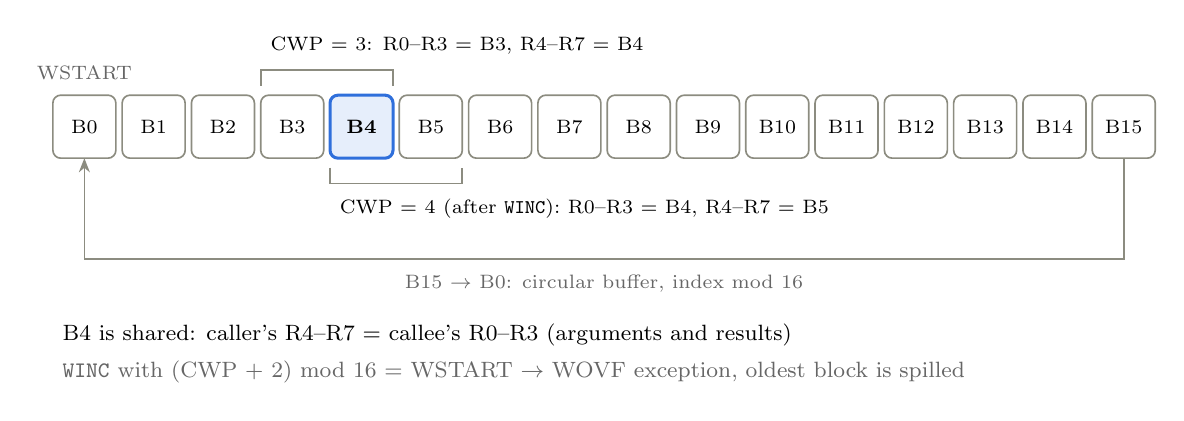
\begin{tikzpicture}[
    x=0.2mm, y=-0.2mm,
    >={Stealth[length=1.8mm,width=1.4mm]},
    conn/.style={draw=lineclr, line width=0.6pt},
    lbl/.style={font=\scriptsize},
  ]
  % --- 16 blocks ------------------------------------------------------
  \foreach \i in {0,...,15} {
    \pgfmathsetmacro{\bx}{24+44*\i}
    \ifnum\i=4
      \draw[draw=accent, fill=accent!12, line width=1.1pt, rounded corners=1mm]
        (\bx,96) rectangle ++(40,40);
      \node[font=\scriptsize\bfseries] at (\bx+20,116) {B\i};
    \else
      \draw[draw=lineclr, line width=0.6pt, rounded corners=1mm]
        (\bx,96) rectangle ++(40,40);
      \node[font=\scriptsize] at (\bx+20,116) {B\i};
    \fi
  }

  % --- window CWP = 3 (blocks 3, 4) -----------------------------------
  \draw[conn] (156,90) -- (156,80) -- (240,80) -- (240,90);
  \node[lbl, anchor=south west] at (156,76) {CWP = 3: R0--R3 = B3, R4--R7 = B4};

  % --- window CWP = 4 (blocks 4, 5) -----------------------------------
  \draw[conn] (200,142) -- (200,152) -- (284,152) -- (284,142);
  \node[lbl, anchor=north west] at (200,156) {CWP = 4 (after \texttt{WINC}): R0--R3 = B4, R4--R7 = B5};

  % --- WSTART marker --------------------------------------------------
  \node[lbl, text=black!60, anchor=south] at (44,92) {WSTART};

  % --- circular wrap-around -------------------------------------------
  \draw[conn,->] (704,136) -- (704,200) -- (44,200) -- (44,136);
  \node[lbl, text=black!60, anchor=north] at (374,204)
    {B15 $\rightarrow$ B0: circular buffer, index mod 16};

  % --- notes ----------------------------------------------------------
  \node[font=\footnotesize, anchor=west] at (24,248)
    {B4 is shared: caller's R4--R7 = callee's R0--R3 (arguments and results)};
  \node[font=\footnotesize, text=black!60, anchor=west] at (24,272)
    {\texttt{WINC} with (CWP + 2) mod 16 = WSTART $\rightarrow$ WOVF exception, oldest block is spilled};
\end{tikzpicture}

  \caption{Register windows: 16 blocks of 4 registers, adjacent windows share one block}
  \label{fig:windows}
\end{figure}

Each window occupies two consecutive blocks, so \texttt{WINC} allocates one new
block while the other stays shared with the caller's window.

\subsection{Calling convention}

\begin{enumerate}
  \item The caller places up to 4 arguments in R4--R7 and executes
        \texttt{CALLW} (= \texttt{WINC} + \texttt{CALL}).
  \item The callee sees the arguments in R0--R3; R4--R7 are its working
        registers and, at the same time, the argument area for further calls.
  \item The callee returns results in R0--R3 and executes \texttt{RETW}
        (= \texttt{WDEC} + \texttt{RET}); the caller reads them in R4--R7.
  \item More than 4 arguments are passed on the stack.
\end{enumerate}

\subsection{Requirements}

\begin{reqtable}
\req{REG-001}{The processor \MUST{} have 64 general-purpose 8-bit registers
  (P0--P63).}
\req{REG-002}{At any time, 8 registers R0--R7 \MUST{} be visible, mapped
  according to Equation~\eqref{eq:window}.}
\req{REG-003}{The window pointer CWP \MUST{} be 4 bits wide (16 positions) and
  \MUST{} be updated modulo 16.}
\req{REG-004}{The \texttt{WINC} instruction \MUST{} increment CWP by 1 (the
  window moves up by 4 registers); \texttt{WDEC} \MUST{} decrement it by 1.}
\req{REG-005}{The register file \MUST{} support two reads and one write in a
  single cycle.}
\req{REG-006}{Register pairs (R0:R1, R2:R3, R4:R5, R6:R7) \MUST{} be usable as
  16-bit address pointers, with the low byte in the even register.}
\req{REG-007}{The register WSTART (4 bits) \MUST{} point to the oldest window
  whose contents are still held in the register file.}
\req{REG-008}{Executing \texttt{WINC} when $(\mathrm{CWP} + 2) \bmod 16 =
  \mathrm{WSTART}$ \MUST{} raise the window overflow exception (WOVF) before
  CWP is changed. This allows up to 15 simultaneously live windows (14 nested
  calls) without spilling to memory.}
\req{REG-009}{Executing \texttt{WDEC} when $\mathrm{CWP} = \mathrm{WSTART}$
  \MUST{} raise the window underflow exception (WUNF) before CWP is changed.}
\req{REG-010}{After a WOVF/WUNF handler returns (\texttt{RETI}), the
  instruction that raised the exception \MUST{} be executed again.}
\req{REG-011}{The exception handler \MUST{} be able to access any physical
  register through the SFRs PRIDX (index 0--63) and PRDAT (data), in order to
  save the WSTART block to the stack (spill) or restore it (fill).}
\req{REG-012}{Register contents after reset \MAY{} be undefined; the
  implementation \SHOULD{} clear them in simulation to simplify debugging.}
\end{reqtable}

% =====================================================================
\section{Special function registers and flags}
\label{sec:sfr}
% =====================================================================

Control and peripheral registers reside in the 8-bit SFR address space, which
is reachable through the SFR addressing mode of every two-operand instruction
(e.g.\ \texttt{OR R1, [SFR:I2CCON]}). Peripherals are therefore operated with
the same instructions as memory.

\subsection{SFR map}

{\small
\begin{xltabular}{\linewidth}{@{}l l l l X@{}}
  \toprule
  \textbf{Address} & \textbf{Name} & \textbf{Access} & \textbf{Reset} & \textbf{Description} \\
  \midrule
  \endfirsthead
  \toprule
  \textbf{Address} & \textbf{Name} & \textbf{Access} & \textbf{Reset} & \textbf{Description} \\
  \midrule
  \endhead
  \bottomrule
  \endfoot
  \hex{00} & SR      & R/W   & \hex{00} & Status register (flags, IE), see \ref{sec:sr} \\
  \hex{01} & SPL     & R/W   & see \reqref{INT-011} & Stack pointer, low byte \\
  \hex{02} & SPH     & R/W   & see \reqref{INT-011} & Stack pointer, high byte \\
  \hex{03} & CWP     & R/W   & \hex{00} & Bits 3:0: current register window \\
  \hex{04} & WSTART  & R/W   & \hex{00} & Bits 3:0: oldest window held in the register file \\
  \hex{05} & PRIDX   & R/W   & \hex{00} & Bits 5:0: physical register index \\
  \hex{06} & PRDAT   & R/W   & --       & Read/write of physical register P[PRIDX] \\
  \hex{08} & INTEN   & R/W   & \hex{00} & Maskable interrupt enable (bit 0 INT0, bit 1 \IIC) \\
  \hex{09} & INTFLG  & R/W1C & \hex{00} & Pending interrupt flags; writing 1 clears \\
  \hex{10} & I2CCON  & R/W   & \hex{00} & \IIC{} controller control, see Section~\ref{sec:i2c} \\
  \hex{11} & I2CSTA  & R/W1C & \hex{00} & \IIC{} controller status \\
  \hex{12} & I2CADR  & R/W   & \hex{00} & Bits 6:0: 7-bit slave address \\
  \hex{13} & I2CTXD  & W     & \hex{00} & Byte to transmit \\
  \hex{14} & I2CRXD  & R     & \hex{00} & Last received byte \\
  \hex{15} & I2CBRG  & R/W   & \hex{FF} & SCL clock divider \\
  \multicolumn{4}{@{}l}{\hex{07}, \hex{0A}--\hex{0F}, \hex{16}--\hex{FF}} & Reserved; reads return \hex{00}, writes are ignored \\
\end{xltabular}
}

\subsection{Status register SR}
\label{sec:sr}

\begin{center}
\small
\begin{tabularx}{0.85\linewidth}{@{}l l X@{}}
  \toprule
  \textbf{Bit} & \textbf{Name} & \textbf{Meaning} \\
  \midrule
  0   & C  & Carry / borrow; for \IIC{} instructions: transaction error \\
  1   & Z  & Result is zero \\
  2   & N  & Bit 7 of the result (sign) \\
  3   & V  & Signed (two's complement) overflow \\
  4--6 & -- & Reserved, read as 0 \\
  7   & IE & Global enable for maskable interrupts \\
  \bottomrule
\end{tabularx}
\end{center}

\subsection{Requirements}

\begin{reqtable}
\req{SFR-001}{The SFR address space \MUST{} contain 256 addresses (8 bits) and
  \MUST{} be separate from data memory.}
\req{SFR-002}{The SFRs \MUST{} be implemented as listed in the SFR map,
  including their reset values.}
\req{SFR-003}{A read from a reserved address \MUST{} return \hex{00}; a write
  to it \MUST{} be ignored without raising an exception.}
\req{SFR-004}{Bits marked R/W1C \MUST{} be cleared by writing 1; writing 0
  \MUST{} leave them unchanged.}
\req{SFR-005}{SPL/SPH \SHOULD{} be written in the order SPL, SPH; the
  implementation \MAY{} block interrupts for one instruction after a write to
  SPL to avoid an inconsistent SP.}
\req{SFR-006}{ALU instructions \MUST{} update the flags as listed in the
  ``Flags'' column of the instruction tables (Section~\ref{sec:isa}); all other
  instructions \MUSTNOT{} change the flags unless stated otherwise.}
\end{reqtable}

% =====================================================================
\section{Instruction set architecture (ISA)}
\label{sec:isa}
% =====================================================================

Instructions are 1--4 bytes long: an opcode byte, an optional operand
specifier byte and 0--2 extension bytes (immediate, displacement or address).
The CISC core consists of 11 two-operand operations, each available in 7
addressing modes, including memory as the destination.

\subsection{Instruction formats}

\begin{center}
\small
\begin{tabularx}{\linewidth}{@{}l l l l X@{}}
  \toprule
  \textbf{Format} & \textbf{Byte 0} & \textbf{Byte 1} & \textbf{Bytes 2--3} & \textbf{Used for} \\
  \midrule
  A & opcode & --        & --                        & No operands (\texttt{NOP}, \texttt{RET}, \texttt{EI}, \ldots) \\
  B & opcode & specifier & --                        & Register / register pair \\
  C & opcode & specifier & imm8 / disp8 / addr8      & Immediate, displacement, SFR address \\
  D & opcode & specifier & addr16 (LSB, MSB)         & Direct address \\
  E & opcode & rel8 / addr16 LSB & addr16 MSB       & Jumps and calls (2 B with rel8, 3 B with addr16) \\
  \bottomrule
\end{tabularx}
\end{center}

For the two-operand group (opcodes \hex{00}--\hex{7F}) the opcode byte holds the
operation number OP in bits 7:3 and the addressing mode MODE in bits 2:0. The
specifier byte holds Rd in bits 7:5, Rs in bits 4:2 (for indirect modes: the
even number of the register pair), the direction bit D in bit 1
(0: result in Rd, 1: result in operand M) and a reserved 0 in bit 0
(Figure~\ref{fig:format}).

\begin{figure}[htbp]
  \centering
  % ---------------------------------------------------------------------
%  Two-operand instruction encoding: opcode byte + specifier byte
%  One bit = 36 units, 1 unit = 0.2 mm, y grows downwards.
%  \field{byte x0}{msb}{lsb}{label}{style}
% ---------------------------------------------------------------------
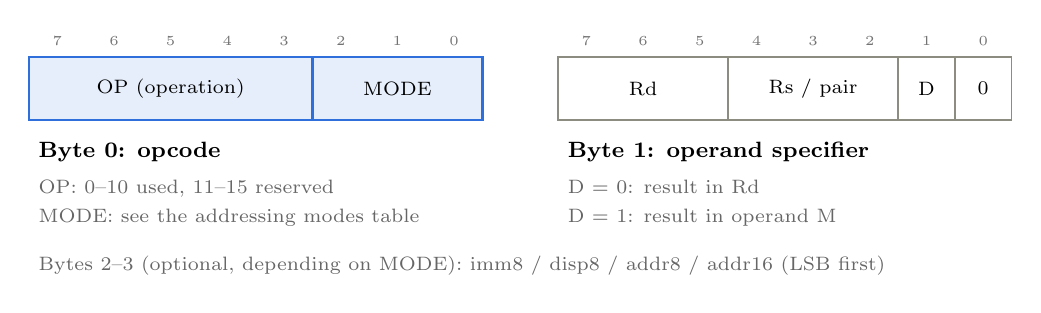
\begin{tikzpicture}[
    x=0.2mm, y=-0.2mm,
    fld/.style={draw=lineclr, line width=0.6pt},
    hl/.style={draw=accent, fill=accent!12, line width=0.9pt},
    bitno/.style={font=\tiny, text=black!55},
  ]
  \newcommand{\field}[5]{%
    \pgfmathsetmacro{\fx}{#1+36*(7-#2)}
    \pgfmathsetmacro{\fw}{36*(#2-#3+1)}
    \draw[#5] (\fx,60) rectangle ++(\fw,40);
    \node[font=\scriptsize] at (\fx+\fw/2,80) {#4};
  }

  % --- bit numbers ----------------------------------------------------
  \foreach \b in {0,...,7} {
    \node[bitno] at (24+36*7-36*\b+18,50)  {\b};
    \node[bitno] at (360+36*7-36*\b+18,50) {\b};
  }

  % --- byte 0: opcode -------------------------------------------------
  \field{24}{7}{3}{OP (operation)}{hl}
  \field{24}{2}{0}{MODE}{hl}
  \node[font=\footnotesize\bfseries, anchor=north west] at (24,108) {Byte 0: opcode};

  % --- byte 1: operand specifier --------------------------------------
  \field{360}{7}{5}{Rd}{fld}
  \field{360}{4}{2}{Rs / pair}{fld}
  \field{360}{1}{1}{D}{fld}
  \field{360}{0}{0}{0}{fld}
  \node[font=\footnotesize\bfseries, anchor=north west] at (360,108) {Byte 1: operand specifier};

  % --- notes ----------------------------------------------------------
  \node[font=\scriptsize, text=black!60, anchor=north west] at (24,132)  {OP: 0--10 used, 11--15 reserved};
  \node[font=\scriptsize, text=black!60, anchor=north west] at (24,150)  {MODE: see the addressing modes table};
  \node[font=\scriptsize, text=black!60, anchor=north west] at (360,132) {D = 0: result in Rd};
  \node[font=\scriptsize, text=black!60, anchor=north west] at (360,150) {D = 1: result in operand M};
  \node[font=\scriptsize, text=black!60, anchor=north west] at (24,180)
    {Bytes 2--3 (optional, depending on MODE): imm8 / disp8 / addr8 / addr16 (LSB first)};
\end{tikzpicture}

  \caption{Encoding of a two-operand instruction (opcode = OP $\cdot$ 8 + MODE)}
  \label{fig:format}
\end{figure}

\subsection{Addressing modes}

\begin{center}
\small
\begin{tabularx}{\linewidth}{@{}l l X l l@{}}
  \toprule
  \textbf{MODE} & \textbf{Name} & \textbf{Operand M} & \textbf{D=1 allowed} & \textbf{Length} \\
  \midrule
  000 & Register              & Rs                                   & no  & 2 B \\
  001 & Immediate             & imm8                                 & no  & 3 B \\
  010 & Direct                & mem[addr16]                          & yes & 4 B \\
  011 & Indirect              & mem[Rs+1:Rs]                         & yes & 2 B \\
  100 & Indirect post-increment & mem[pair], then pair $\leftarrow$ pair + 1 & yes & 2 B \\
  101 & --                    & Reserved (ILL exception)             & --  & -- \\
  110 & Indexed               & mem[pair + signed disp8]             & yes & 3 B \\
  111 & SFR                   & sfr[addr8]                           & yes & 3 B \\
  \bottomrule
\end{tabularx}
\end{center}

\subsection{Two-operand operations}

\begin{center}
\small
\begin{tabularx}{\linewidth}{@{}l l X l@{}}
  \toprule
  \textbf{OP} & \textbf{Mnemonic} & \textbf{Operation (D=0)} & \textbf{Flags} \\
  \midrule
  0  & \texttt{MOV} & Rd $\leftarrow$ M                         & Z, N \\
  1  & \texttt{ADD} & Rd $\leftarrow$ Rd + M                    & C, Z, N, V \\
  2  & \texttt{ADC} & Rd $\leftarrow$ Rd + M + C                & C, Z, N, V \\
  3  & \texttt{SUB} & Rd $\leftarrow$ Rd $-$ M                  & C, Z, N, V \\
  4  & \texttt{SBC} & Rd $\leftarrow$ Rd $-$ M $-$ C            & C, Z, N, V \\
  5  & \texttt{AND} & Rd $\leftarrow$ Rd $\wedge$ M             & Z, N; V = 0 \\
  6  & \texttt{OR}  & Rd $\leftarrow$ Rd $\vee$ M               & Z, N; V = 0 \\
  7  & \texttt{XOR} & Rd $\leftarrow$ Rd $\oplus$ M             & Z, N; V = 0 \\
  8  & \texttt{CMP} & Rd $-$ M, flags only                      & C, Z, N, V \\
  9  & \texttt{TST} & Rd $\wedge$ M, flags only                 & Z, N; V = 0 \\
  10 & \texttt{MUL} & Rd+1:Rd $\leftarrow$ Rd $\times$ M (unsigned); Rd even, D = 0 & Z (16-bit result), C = high byte $\neq$ 0 \\
  11--15 & -- & Reserved (ILL exception) & -- \\
  \bottomrule
\end{tabularx}
\end{center}

With D=1 the result is written to M; for example \texttt{ADD [0x0420], R3}
adds R3 to a memory location (read--modify--write in a single instruction).
For \texttt{MOV} with D=1: M $\leftarrow$ Rd.

\subsection{Other instructions}

{\small
\begin{xltabular}{\linewidth}{@{}l >{\raggedright\arraybackslash}p{4.3cm} l >{\raggedright\arraybackslash}X@{}}
  \toprule
  \textbf{Opcode} & \textbf{Mnemonic} & \textbf{Format} & \textbf{Operation} \\
  \midrule
  \endfirsthead
  \toprule
  \textbf{Opcode} & \textbf{Mnemonic} & \textbf{Format} & \textbf{Operation} \\
  \midrule
  \endhead
  \bottomrule
  \endfoot
  \hex{80}--\hex{89} & \texttt{INC, DEC, NEG, NOT, CLR, SHL, SHR, ASR, RLC, RRC} & B (Rd) & Single-operand operations on Rd \\
  \hex{8D} / \hex{8E} & \texttt{PUSH Rd} / \texttt{POP Rd} & B & SP $\leftarrow$ SP$-$1, mem[SP] $\leftarrow$ Rd / Rd $\leftarrow$ mem[SP], SP $\leftarrow$ SP+1 \\
  \hex{8F} / \hex{90} & \texttt{INCW} / \texttt{DECW} & B (pair) & 16-bit increment / decrement of a pair, flag Z \\
  \hex{91} & \texttt{LPM Rd, [pair]} & B & Rd $\leftarrow$ program memory[pair] (\reqref{MEM-005}) \\
  \hex{B0}--\hex{B5} & \texttt{JZ, JNZ, JC, JNC, JN, JNN} & E (rel8) & Conditional relative jump, $-128 \ldots +127$ \\
  \hex{B9} & \texttt{JMP addr16} & E & Unconditional jump \\
  \hex{BB} & \texttt{CALL addr16} & E & Push PC and jump \\
  \hex{BD} & \texttt{DJNZ Rd, rel8} & C & Rd $\leftarrow$ Rd $-$ 1; jump if Rd $\neq$ 0 \\
  \hex{BE} & \texttt{CALLW addr16} & E & \texttt{WINC}, then \texttt{CALL} \\
  \hex{C0} / \hex{C1} / \hex{C2} & \texttt{RET} / \texttt{RETI} / \texttt{RETW} & A & Return / return from interrupt / \texttt{WDEC} + \texttt{RET} \\
  \hex{C3} / \hex{C4} & \texttt{WINC} / \texttt{WDEC} & A & Move window by $+4$ / $-4$ registers \\
  \hex{C5} / \hex{C6} & \texttt{PUSHF} / \texttt{POPF} & A & Push / pop SR \\
  \hex{C7} / \hex{C8} & \texttt{EI} / \texttt{DI} & A & IE $\leftarrow$ 1 / IE $\leftarrow$ 0 \\
  \hex{C9} & \texttt{HALT} & A & Sleep until interrupt \\
  \hex{D0} & \texttt{I2CW Ra, Rd} & B & Write byte Rd to slave at address Ra (Section~\ref{sec:i2c-hl}) \\
  \hex{D1} & \texttt{I2CR Rd, Ra} & B & Read one byte from slave Ra into Rd \\
  \hex{D2} & \texttt{I2CRR Rd, Ra} & B & Register read: Ra = slave address, Ra+1 = register number (repeated START) \\
  \hex{D3} & \texttt{I2CRRN [pair], Ra, \#n} & C (imm8 = n) & Read n bytes starting at register Ra+1 of slave Ra into data memory at [pair], pair $\leftarrow$ pair + n \\
  \hex{D4} & \texttt{I2CWN [pair], Ra, \#n} & C (imm8 = n) & Write n bytes from data memory at [pair] to slave Ra, pair $\leftarrow$ pair + n \\
  \hex{F0} & \texttt{NOP} & A & No operation \\
  \hex{FF} & \texttt{TRAP} & A & Software exception (ILL vector); \hex{FF} = erased memory \\
  others & -- & -- & Reserved, ILL exception \\
\end{xltabular}
}

\subsection{Requirements}

\begin{reqtable}
\req{ISA-001}{The processor \MUST{} implement all instructions listed in the
  instruction tables, with the specified encoding.}
\req{ISA-002}{Every two-operand operation \MUST{} work in all 7 addressing
  modes; MODE = 101 is reserved and \MUST{} raise the ILL exception.}
\req{ISA-003}{D=1 combined with the register or immediate mode, \texttt{MUL}
  with D=1 or an odd Rd, and an indirect mode with an odd Rs \MUST{} raise the
  ILL exception.}
\req{ISA-004}{Instructions with D=1 \MUST{} perform the read--modify--write of
  the memory operand as an atomic operation (no interrupt is taken in
  between).}
\req{ISA-005}{Relative jumps \MUST{} compute the target relative to the
  address of the next instruction.}
\req{ISA-006}{\texttt{CALL} \MUST{} push the 16-bit return address onto the
  stack (high byte first, so that the low byte ends up at the lower address).}
\req{ISA-007}{The number of clock cycles for every instruction and addressing
  mode \MUST{} be documented in the appendix ``Instruction timing table''.}
\req{ISA-040}{The instructions \texttt{I2CW}, \texttt{I2CR}, \texttt{I2CRR},
  \texttt{I2CRRN} and \texttt{I2CWN} \MUST{} stall execution until the
  transaction completes or times out, and \MUST{} set C = 1 on error (NACK,
  arbitration lost, timeout).}
\req{ISA-041}{For \texttt{I2CRRN} and \texttt{I2CWN} the pair \MUST{} be given
  by its even register number in the Rd field and Ra in the Rs field; an odd
  pair number or n = 0 \MUST{} raise the ILL exception. After the instruction
  the pair \MUST{} point just past the last byte actually transferred (also
  when the transaction is aborted by an error).}
\req{ISA-050}{Opcode \hex{FF} and every reserved opcode \MUST{} raise the ILL
  exception; the saved PC points to that instruction.}
\end{reqtable}

% =====================================================================
\section{\texorpdfstring{\IIC{}}{I2C} controller}
\label{sec:i2c}
% =====================================================================

The \IIC{} controller operates as a bus master (7-bit addressing, 100 and
400\,kHz) and offers two levels of use: six SFRs for full control of a
transaction, and five high-level instructions (\texttt{I2CW},
\texttt{I2CR}, \texttt{I2CRR}, and the multi-byte \texttt{I2CRRN},
\texttt{I2CWN}) that cover the common cases in a single line of code.

\subsection{Rationale for the register set}

Three registers alone (slave address, byte to send, received byte) are enough
to write or read a single byte, but they do not allow:

\begin{itemize}
  \item reading a sensor register, which requires writing the register number
        followed by a \textbf{repeated START} without a STOP;
  \item multi-byte transactions (e.g.\ an EEPROM page write, reading 6 bytes
        from an accelerometer);
  \item error detection: missing ACK (device not responding), arbitration
        lost, a stuck bus;
  \item setting the SCL frequency and checking whether a transfer has finished.
\end{itemize}

The three registers are therefore kept (I2CADR, I2CTXD, I2CRXD), and a
control, a status and a clock divider register are added.

\subsection{Registers}

\needspace{14\baselineskip}
\paragraph{I2CCON (\hex{10})}

\begin{center}
\small
\begin{tabularx}{\linewidth}{@{}l l X@{}}
  \toprule
  \textbf{Bit} & \textbf{Name} & \textbf{Meaning} \\
  \midrule
  7 & EN    & Controller enable \\
  6 & IE    & Interrupt when an operation completes (DONE) \\
  5 & START & Write 1: START (or repeated START if the bus is already owned)
              followed by the address byte \{I2CADR, RW\}; cleared by hardware \\
  4 & STOP  & Write 1: STOP condition; cleared by hardware \\
  3 & RD    & Write 1: receive one byte into I2CRXD; cleared by hardware \\
  2 & ACKS  & Acknowledge sent after a received byte: 0 = ACK, 1 = NACK (last byte) \\
  1 & RW    & Direction in the address phase: 0 = write, 1 = read \\
  0 & --    & Reserved \\
  \bottomrule
\end{tabularx}
\end{center}

\needspace{14\baselineskip}
\paragraph{I2CSTA (\hex{11})}

\begin{center}
\small
\begin{tabularx}{\linewidth}{@{}l l X@{}}
  \toprule
  \textbf{Bit} & \textbf{Name} & \textbf{Meaning} \\
  \midrule
  0 & TIP   & Byte transfer in progress \\
  1 & DONE  & Operation complete (R/W1C); interrupt source \\
  2 & NACK  & The slave did not acknowledge the last byte \\
  3 & ARBL  & Arbitration lost (R/W1C) \\
  4 & BB    & Bus busy (between START and STOP) \\
  5 & RXRDY & New byte in I2CRXD; cleared by reading I2CRXD \\
  6 & TOUT  & Timeout expired (R/W1C) \\
  7 & --    & Reserved \\
  \bottomrule
\end{tabularx}
\end{center}

Writing I2CTXD while BB = 1 starts transmission of that byte. The SCL
frequency is
\begin{equation}
  f_{\mathrm{SCL}} = \frac{f_{\mathrm{CLK}}}{4 \cdot (\mathrm{I2CBRG} + 1)}
  \label{eq:scl}
\end{equation}

Example for $f_{\mathrm{CLK}} = 16$\,MHz: I2CBRG = 39 gives 100\,kHz,
I2CBRG = 9 gives 400\,kHz.

\subsection{High-level instructions}
\label{sec:i2c-hl}

\begin{center}
\small
\begin{tabularx}{\linewidth}{@{}l X@{}}
  \toprule
  \textbf{Instruction} & \textbf{Bus sequence} \\
  \midrule
  \texttt{I2CW Ra, Rd}  & START, address(Ra)+W, byte Rd, STOP \\
  \texttt{I2CR Rd, Ra}  & START, address(Ra)+R, byte $\rightarrow$ Rd (NACK), STOP \\
  \texttt{I2CRR Rd, Ra} & START, address(Ra)+W, byte Ra+1, repeated START,
                          address(Ra)+R, byte $\rightarrow$ Rd (NACK), STOP \\
  \texttt{I2CRRN [pair], Ra, \#n} & START, address(Ra)+W, byte Ra+1, repeated START,
                          address(Ra)+R, n bytes $\rightarrow$ mem[pair\ldots pair+n$-$1]
                          (ACK after each byte, NACK after the last), STOP \\
  \texttt{I2CWN [pair], Ra, \#n} & START, address(Ra)+W, n bytes from
                          mem[pair\ldots pair+n$-$1], STOP \\
  \bottomrule
\end{tabularx}
\end{center}

The multi-byte instructions transfer data directly between the \IIC{}
controller and data memory; the bytes are stored in bus order at increasing
addresses. To write device registers with \texttt{I2CWN}, the first byte of
the buffer holds the register number. Because the processor stalls for the
whole transaction (about 9 SCL periods per byte: roughly 0.8\,ms for 6 bytes
at 100\,kHz), longer transfers \SHOULD{} use 400\,kHz.

Example: reading 6 bytes (registers \hex{3B}--\hex{40}) from an
accelerometer at address \hex{68} into a buffer:

\begin{lstlisting}
    MOV    R2, #0x68        ; slave address
    MOV    R3, #0x3B        ; first register
    MOV    R4, #<buf        ; R5:R4 = buffer address
    MOV    R5, #>buf
    I2CRRN [R4], R2, #6     ; buf[0..5] <- registers 0x3B..0x40
    JC     i2c_error
\end{lstlisting}

\begin{figure}[htbp]
  \centering
  % ---------------------------------------------------------------------
%  I2C frame generated by I2CRR
%  Each field: x / width / driven-by-slave (1|0) / label
%  1 unit = 0.2 mm, y grows downwards.
% ---------------------------------------------------------------------
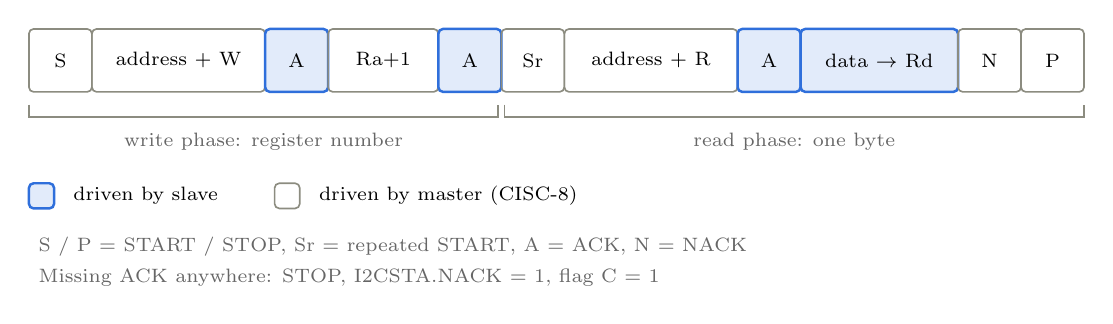
\begin{tikzpicture}[
    x=0.2mm, y=-0.2mm,
    conn/.style={draw=lineclr, line width=0.6pt},
    lbl/.style={font=\scriptsize, text=black!60},
    master/.style={draw=lineclr, line width=0.6pt, rounded corners=0.6mm},
    slave/.style={draw=accent, fill=accent!14, line width=0.9pt, rounded corners=0.6mm},
  ]
  \foreach \x/\w/\s/\t in {
      24/40/0/S,
      64/110/0/{address + W},
      174/40/1/A,
      214/70/0/Ra+1,
      284/40/1/A,
      324/40/0/Sr,
      364/110/0/{address + R},
      474/40/1/A,
      514/100/1/{data $\rightarrow$ Rd},
      614/40/0/N,
      654/40/0/P} {
    \ifnum\s=1
      \draw[slave] (\x,72) rectangle ++(\w,40);
    \else
      \draw[master] (\x,72) rectangle ++(\w,40);
    \fi
    \node[font=\scriptsize] at (\x+\w/2,92) {\t};
  }

  % --- phases ---------------------------------------------------------
  \draw[conn] (24,120) -- (24,128) -- (322,128) -- (322,120);
  \node[lbl, anchor=north] at (173,132) {write phase: register number};
  \draw[conn] (326,120) -- (326,128) -- (694,128) -- (694,120);
  \node[lbl, anchor=north] at (510,132) {read phase: one byte};

  % --- legend ---------------------------------------------------------
  \draw[slave]  (24,170)  rectangle ++(16,16);
  \node[font=\scriptsize, anchor=west] at (46,178)  {driven by slave};
  \draw[master] (180,170) rectangle ++(16,16);
  \node[font=\scriptsize, anchor=west] at (202,178) {driven by master (CISC-8)};

  \node[lbl, anchor=west] at (24,210)
    {S / P = START / STOP, Sr = repeated START, A = ACK, N = NACK};
  \node[lbl, anchor=west] at (24,230)
    {Missing ACK anywhere: STOP, I2CSTA.NACK = 1, flag C = 1};
\end{tikzpicture}

  \caption{\IIC{} frame generated by \texttt{I2CRR}: register number write, repeated START, single-byte read}
  \label{fig:i2cframe}
\end{figure}

The repeated START (Sr) keeps ownership of the bus between writing the
register number and reading the data, so no other master can intervene
(Figure~\ref{fig:i2cframe}).

Example: reading register \hex{75} from a sensor at address \hex{68}:

\begin{lstlisting}
    MOV   R2, #0x68     ; slave address
    MOV   R3, #0x75     ; register number
    I2CRR R0, R2        ; R0 <- data read
    JC    i2c_error     ; C = 1: NACK / timeout
\end{lstlisting}

\subsection{Requirements}

\begin{reqtable}
\req{I2C-001}{The controller \MUST{} operate as a master only, with 7-bit
  addressing, in accordance with NXP UM10204. Slave mode and 10-bit
  addressing are not supported.}
\req{I2C-002}{The controller \MUST{} support Standard mode (100\,kHz) and Fast
  mode (400\,kHz); the frequency is set by I2CBRG according to
  Equation~\eqref{eq:scl}.}
\req{I2C-003}{The controller \MUST{} generate START, repeated START and STOP
  conditions, and transmit and receive bytes with ACK/NACK handling.}
\req{I2C-004}{The controller \MUST{} support clock stretching by the slave by
  sampling the SCL line.}
\req{I2C-005}{The controller \MUST{} detect arbitration loss (SDA read back
  differs from SDA driven), release the bus and set ARBL.}
\req{I2C-006}{The controller \MUST{} abort the operation and set TOUT when SCL
  is held low longer than the timeout (synthesis parameter, default 25\,ms).}
\req{I2C-007}{SDA and SCL \MUST{} be driven as open-drain (low or
  high-impedance only); the pull-up resistors are external.}
\req{I2C-008}{The SDA and SCL inputs \MUST{} be synchronised to CLK (at least
  2 flip-flops) and \SHOULD{} have a glitch filter suppressing pulses shorter
  than 50\,ns.}
\req{I2C-009}{Setting DONE while IE = 1 \MUST{} raise the \IIC{} interrupt.}
\req{I2C-010}{The instructions \texttt{I2CW}, \texttt{I2CR}, \texttt{I2CRR},
  \texttt{I2CRRN} and \texttt{I2CWN} \MUST{} use the same controller and
  leave the final status in I2CSTA.}
\req{I2C-011}{For \texttt{I2CRRN} and \texttt{I2CWN} the controller \MUST{}
  read and write data memory directly, one byte per transferred \IIC{} byte
  (\reqref{ISA-041}).}
\end{reqtable}

% =====================================================================
\section{Interrupts, exceptions and reset}
\label{sec:int}
% =====================================================================

The processor has three non-maskable exceptions (WOVF, WUNF, ILL) and two
maskable interrupts (INT0, \IIC), served through a fixed vector table at the
start of program memory; the user program starts at \hex{0020}.

\subsection{Vector table}

\begin{center}
\small
\begin{tabularx}{\linewidth}{@{}l X l l@{}}
  \toprule
  \textbf{Address} & \textbf{Source} & \textbf{Type} & \textbf{Priority} \\
  \midrule
  \hex{0000} & RESET & -- & highest \\
  \hex{0004} & WOVF: register window overflow & exception, non-maskable & 1 \\
  \hex{0008} & WUNF: register window underflow & exception, non-maskable & 2 \\
  \hex{000C} & ILL: illegal instruction / \texttt{TRAP} & exception, non-maskable & 3 \\
  \hex{0010} & INT0: external interrupt & maskable & 4 \\
  \hex{0014} & \IIC: operation complete & maskable & 5 \\
  \hex{0018}--\hex{001F} & Reserved & -- & -- \\
  \bottomrule
\end{tabularx}
\end{center}

Each vector is 4 bytes long, which fits a \texttt{JMP addr16} instruction (3 bytes).

\subsection{Requirements}

\begin{reqtable}
\req{INT-001}{A maskable interrupt \MUST{} be taken only when SR.IE = 1, its
  bit in INTEN is set and its flag in INTFLG is set.}
\req{INT-002}{Interrupts \MUST{} be taken only between instructions;
  exceptions (WOVF, WUNF, ILL) are raised before execution of the instruction
  that caused them.}
\req{INT-003}{On entry to a handler, the processor \MUST{} push PC (2 bytes)
  and SR (1 byte) onto the stack, clear SR.IE and jump to the vector address.}
\req{INT-004}{For an interrupt, the saved PC \MUST{} point to the next
  instruction; for an exception, to the instruction that raised it.}
\req{INT-005}{\texttt{RETI} \MUST{} pop SR and PC from the stack (restoring IE).}
\req{INT-006}{When several sources are pending, the source with the highest
  priority according to the vector table \MUST{} be served first.}
\req{INT-007}{The latency from the end of the current instruction to the first
  instruction of the handler \SHOULD{} not exceed 8 cycles; the actual value
  \MUST{} be documented.}
\req{INT-008}{The INT0 input \MUST{} be synchronised to CLK; the interrupt is
  triggered on the falling edge.}
\req{INT-009}{A handler that uses \texttt{WINC} \MUST{} execute \texttt{WDEC}
  before \texttt{RETI}; the WOVF/WUNF handlers \MUSTNOT{} use \texttt{WINC} or
  \texttt{WDEC}.}
\req{INT-010}{\texttt{HALT} \MUST{} suspend execution until an interrupt occurs
  (also with IE = 0, in which case execution resumes at the next instruction
  without entering the handler).}
\req{INT-011}{After reset: PC = \hex{0000}, SR = \hex{00}, CWP = WSTART = 0,
  INTEN = INTFLG = 0, \IIC{} controller disabled, SP = \hex{0800} (the
  first \texttt{PUSH} writes the last byte of data memory, \hex{07FF}).}
\req{INT-012}{The \texttt{RST\_N} signal \MUST{} be active low, with
  asynchronous assertion and synchronous de-assertion (2 flip-flops).}
\end{reqtable}

% =====================================================================
\section{External interfaces and non-functional requirements}
\label{sec:io}
% =====================================================================

The core exposes the clock, reset, one interrupt input, the two \IIC{} lines and
the buses of both memories, so that the memories can be either FPGA block RAM
or external devices.

\subsection{Core signals}

\begin{center}
\small
\begin{tabularx}{\linewidth}{@{}l l l X@{}}
  \toprule
  \textbf{Signal} & \textbf{Direction} & \textbf{Width} & \textbf{Description} \\
  \midrule
  \texttt{CLK}     & in     & 1  & System clock \\
  \texttt{RST\_N}  & in     & 1  & Reset, active low (\reqref{INT-012}) \\
  \texttt{INT0\_N} & in     & 1  & External interrupt, falling edge \\
  \texttt{SDA}     & in/out & 1  & \IIC{} data, open-drain \\
  \texttt{SCL}     & in/out & 1  & \IIC{} clock, open-drain \\
  \texttt{P\_ADDR} & out    & 16 & Program memory address \\
  \texttt{P\_DATA} & in     & 8  & Program memory data \\
  \texttt{D\_ADDR} & out    & 16 & Data memory address \\
  \texttt{D\_WDATA}& out    & 8  & Write data \\
  \texttt{D\_RDATA}& in     & 8  & Read data \\
  \texttt{D\_WE}   & out    & 1  & Write enable \\
  \texttt{HALTED}  & out    & 1  & Processor in HALT state (diagnostics) \\
  \bottomrule
\end{tabularx}
\end{center}

\subsection{Interface requirements}

\begin{reqtable}
\req{IO-001}{The core \MUST{} provide the signals listed in the core signal table.}
\req{IO-002}{The memory buses \MUST{} be synchronous with a read latency of
  1 cycle (compatible with block RAM of typical FPGAs).}
\req{IO-003}{A top-level variant with embedded memories and tri-state
  SDA/SCL drivers \MUST{} exist, ready for synthesis on the target board.}
\end{reqtable}

\subsection{Non-functional requirements}

\begin{reqtable}
\req{NF-001}{The design \MUST{} be described in a synthesisable HDL
  (Verilog/SystemVerilog or VHDL -- to be decided).}
\req{NF-002}{The design \MUST{} be fully synchronous: no latches, no gated
  clocks and no combinational loops; it \MUST{} pass lint without critical
  warnings.}
\req{NF-003}{The target clock frequency \SHOULD{} be at least 50\,MHz on the
  selected FPGA (to be confirmed once the device is chosen).}
\req{NF-004}{The \IIC{} timeout and the default value of I2CBRG
  \MUST{} be parameters (generic/parameter) of the top-level module.}
\req{NF-005}{Each block (ALU, register file, control unit, \IIC{} controller,
  interrupt controller) \MUST{} be a separate module with its own testbench.}
\req{NF-006}{The source code \MUST{} be kept under version control.}
\req{NF-007}{The documentation \MUST{} include this specification, a
  microarchitecture description and the instruction timing table.}
\end{reqtable}


\end{document}
